\documentclass[xcolor=x11names,compress,professionalfonts]{beamer}

%% General packages %%%%%%%%%%%%%%%%%%%%%%%%%%%%%%%%%%
\usepackage[utf8]{inputenc}
\usepackage{graphicx}
\usepackage{tikz}
\tikzset{% change default arrow tips
    >=latex
}
\usepackage{ifthen}

\usepackage{amsmath}
\usepackage{nicefrac}

\usepackage{color}

%%%%%%%%%%%%%%%%%%%%%%%%%%%%%%%%%%%%%%%%%%%%%%%%%%%%%%


%% Beamer Layout %%%%%%%%%%%%%%%%%%%%%%%%%%%%%%%%%%
\useoutertheme[subsection=false,shadow]{miniframes}
\useinnertheme{rectangles}

\setbeamertemplate{navigation symbols}{}%remove navigation symbols

\newcommand{\btVFill}{\vskip0pt plus 1filll}%place an element at the bottom of the page

\usepackage{libertine}
\usepackage[T1]{fontenc}

\setbeamerfont{title like}{shape=\scshape}
\setbeamerfont{frametitle}{shape=\scshape}

\setbeamercolor*{lower separation line head}{bg=DeepSkyBlue4} 
\setbeamercolor*{normal text}{fg=black,bg=white} 
\setbeamercolor*{alerted text}{fg=red} 
\setbeamercolor*{example text}{fg=black} 
\setbeamercolor*{structure}{fg=black} 
 
\setbeamercolor*{palette tertiary}{fg=black,bg=black!10} 
\setbeamercolor*{palette quaternary}{fg=black,bg=black!10} 

\renewcommand{\(}{\begin{columns}}
\renewcommand{\)}{\end{columns}}
\newcommand{\<}[1]{\begin{column}{#1}}
\renewcommand{\>}{\end{column}}

% idos
\newcommand{\id}{\ensuremath{\text{idos}}}

\definecolor{BostonBlue}{HTML}{00688B}
\definecolor{Complementary}{HTML}{8B2300}
%%%%%%%%%%%%%%%%%%%%%%%%%%%%%%%%%%%%%%%%%%%%%%%%%%

\usepackage{braket}
% compile child documents using this preamble
\usepackage{subfiles}

%%%My Math

\newcommand{\pd}[2]{\frac{\displaystyle \partial #1}{\displaystyle\partial #2}} % for partial derivatives
\newcommand{\dx}{\mathrm{d}x}
\renewcommand{\d}[1]{\mathrm{d}#1}
\newcommand{\nth}{$n^\text{th}$ }

\newcommand{\mean}[1]{\langle #1 \rangle}
\DeclareMathOperator{\Pf}{Pf}
\DeclareMathOperator{\Tr}{Tr}

\begin{document}


\begin{frame}
\title{{\fontsize{14}{60}\selectfont Gap structure of 1D cut and project Hamiltonians}}

\author{Nicolas Macé, Anuradha Jagannathan, Frédéric Piéchon}

\institute % (optional)
{
  Laboratoire de Physique des Solides\\
  Université Paris-Saclay
}

\date{September 20, 2016}

\titlepage

\btVFill
\begin{columns}
\begin{column}{2cm}
~\\
~\\
~\\
~\\
\raggedright

\includegraphics[scale=.15]{img/LogoUPSUD.png}
\end{column}
\begin{column}{6cm}
\centering
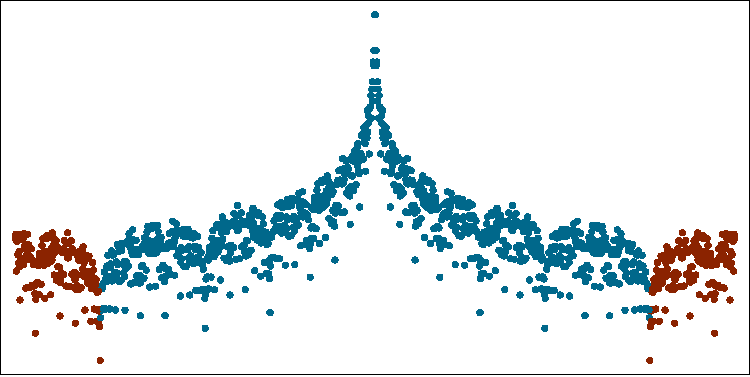
\includegraphics[width=1.\textwidth]{img/cover_illustration.pdf}
\end{column}
\begin{column}{2cm}
~\\
~\\
~\\
~\\
\raggedleft

\includegraphics[scale=.15]{img/logo-lps.jpg}
\end{column}
\end{columns}
\end{frame}

\begin{frame}
\frametitle{Outline}
\tableofcontents[hideallsubsections]
\end{frame}

\section{The gap labeling theorem}
%Each section needs a subsection for the small points on top to show up
\subsection{Dummy}

\begin{frame}{Electrons on quasiperiodic chains}
\begin{columns}
\begin{column}{8.5cm}
	\centering
	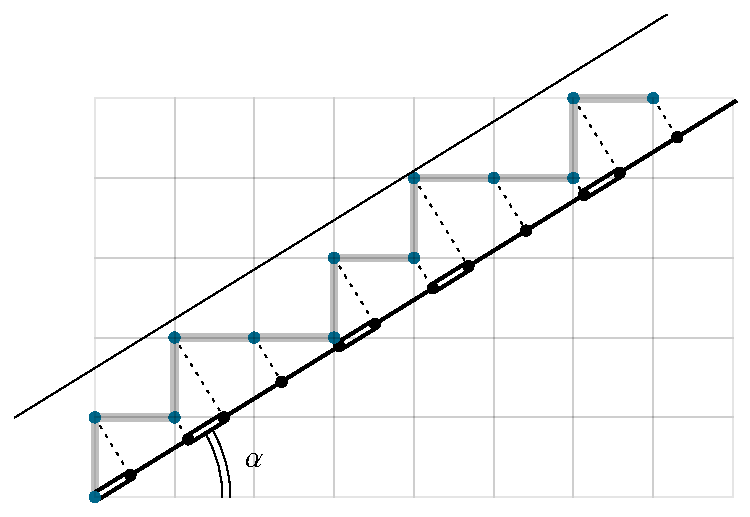
\includegraphics[scale=.7]{img/cut_and_project.pdf}
\end{column}

\begin{column}{3cm}
\begin{align*}
\alpha_l &= \frac{p_l}{q_l} \\
\alpha_l &\rightarrow \alpha
\end{align*}
\end{column}
\end{columns}

	Hamiltonian of the l$^\text{th}$ approximant:
	\[
		H(\alpha) = \sum_{x \in \mathbf{Z}} t_{x,x+1} \ket{x} \bra{x+1} + \text{h.c.}
	\]
\end{frame}

\begin{frame}{The gap labeling theorem}
The IDOS inside spectral gaps can be indexed using the irrational involved in the construction of the chain
	\[
		\id(E \in \text{gap}) = \frac{n}{1+\alpha} \mod 1
	\]


\end{frame}



\end{document}
